\documentclass{bacgost}



% Русские буквы в формулах.
\RequirePackage{mathtext} 

% Для вставки программного кода.
\usepackage{listings}

% "Умная" запятая: \(0,2\) - число, \(0, 2\) - перечисление.
% Можно убрать.
\usepackage{icomma}

% Для рисунков.
\usepackage{tikz}
\usepackage{pgfplots}
\pgfplotsset{compat=newest}

\hypersetup{				
   unicode=true,            % русские буквы в раздела PDF
   colorlinks=false,       	% false: ссылки в рамках; true: цветные ссылки
   linktoc=all,				% ссылки на названиях и номерах страниц в toc
   bookmarksdepth=5,		% глубина закладок в pdf файле
   pdftitle={Заголовок},    % Заголовок
   pdfauthor={Автор},       % Автор
   pdfsubject={Тема},       % Тема
   pdfcreator={Создатель},  % Создатель
   %pdfproducer={Производитель}, % Производитель
   pdfkeywords={keyword1} {key2} {key3} % Ключевые слова
   % linkcolor=blue,        % внутренние ссылки
   % citecolor=black,       % на библиографию
   % filecolor=magenta,     % на файлы
   % urlcolor=cyan          % на URL
} 

\begin{document}


\begin{abstract}
Выпускная квалификационная работа содержит \pageref*{LastPage}~страниц, \total{totfigures}~рисунок, \total{tottables}~таблиц, \total{totappendix}~приложение, \total{totreferences}~источника.
\end{abstract}


\gosttableofcontents


\begin{lofab}
ОДУ - обыкновенные дифференциальные уравнения.

СЛАУ - система линейных алгебраических уравнений.
\end{lofab}


\header{ВВЕДЕНИЕ}
Текст введения.


\mainpart


\section{Первый раздел}
Здесь какой - то текст. Квадратное уравнение.
\begin{equation}
f(x) = x^2 + x-2.
\end{equation}
График представлен на рисунке ниже.
% Важно добавлять каждый рисунок в окружение gostfigure, чтобы был правильный подсчёт общего числа рисунков.
\begin{gostfigure}
\begin{center} 
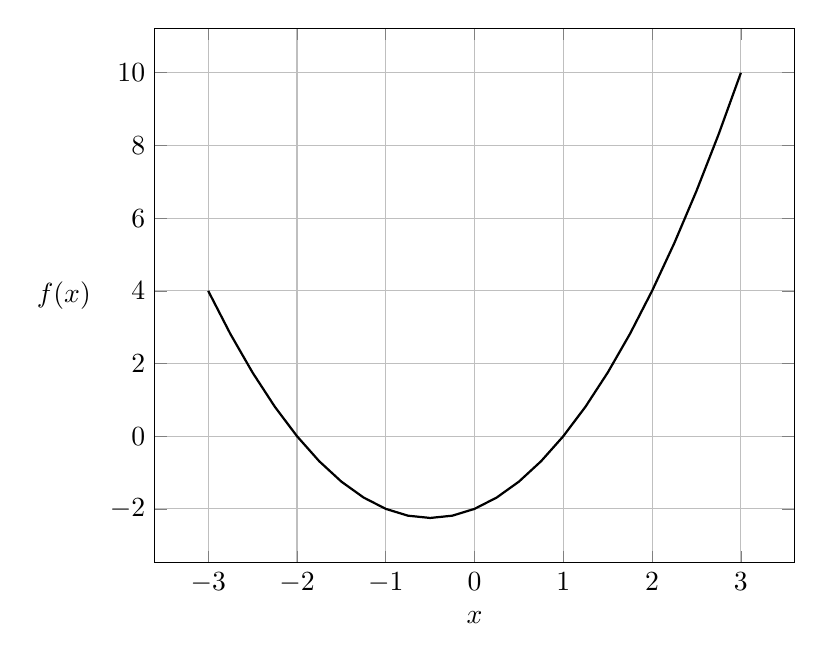
\begin{tikzpicture}
\begin{axis}[domain=-3:3, width = 0.8 \textwidth, grid = both, ylabel style={rotate=-90}, xlabel = \(x\), ylabel = \(f(x)\)]
\addplot[mark=none, thick]{x*x + x - 2};
\end{axis}
\end{tikzpicture}
\captionof{figure}{График \(f(x)\).}
\end{center}
\end{gostfigure}

Корни квадратного уравнения представлены в~таблице. вставлять таблицы.
% Аналогично с таблицами.
\begin{gosttable}
\begin{center} 
\captionof{table}{Корни квадратного уравнения}
\begin{tabular}{|c|c|}
\hline 
Первый корень &  Второй корень \\ 
\hline 
1 & -2  \\ 
\hline 
\end{tabular} 
\end{center}
\end{gosttable}

\subsection{Первый подраздел}

\subsubsection{Ещё один уровень}
\[
\int x\,d\,x = \dfrac{x^2}{2} + C.
\]

\section{Второй раздел}
\[
\dfrac{d\,e^x}{d\,x} = e^x.
\]

\header{ЗАКЛЮЧЕНИЕ}
Интересная статья по нейронным сетям \cite{Cybenko}.


% Список литературы.
\begin{gostbibliography}{11}
\bibitem{Bard} Бард Й. Нелинейное оценивание параметров / Й. Бард, Москва: Статистика, 1979. 349 c.
\bibitem{Volterra} Вольтерра В. Математическая теория борьбы за существование // Усп. физ. наук. 1928. № 1 (8). C. 13–34.
\bibitem{Cybenko} Cybenko G. Approximation by Superpositions of a Sigmoidal Function // Mathematics of Control, Signals, and Systems. 1989. (2). C. 303–314.
\end{gostbibliography}


\begin{gostappendix}{Программный код}
\lstset{language=[11]c++,basicstyle=\ttfamily, showstringspaces=false}

\begin{lstlisting}
#include <iostream>

using namespace std;

int main()
{
  auto b = 1;
  auto a = 2;
  cout << "2 + 1 = " << a + b << endl;
  return 0;
}
\end{lstlisting}

\end{gostappendix}
\end{document}